\documentclass{beamer}

\usepackage{beamer_tom}
\graphicspath{{./images/}}

\def\biblio{
    \nobibliography{../../library}
    \def\biblio{}
}

\institute{INRIA Saclay}
\author{Thomas Moreau}
\title{
    Scketching:\\
    The Jonhson-Linderstrauss Theorem.
}

\setbeamertemplate{title page}[frame]
\def\extraLogo{}

\begin{document}

    \begin{frame}
        \titlepage
    %	\biblio{}
    \end{frame}

    \begin{frame}{Eigenvalues of random covariance matrices}

        Let $X$ denote a matrix in $\mathbb R^{m \times n}$ whose entries $X_{i, j}$ are \emph{i.i.d} with mean $0$ and variance $\sigma^2 < \infty$.
        Consider its covariance matrix
        \[
            Y = \frac1n XX^T
        \] and its eigenvalues $\lambda_1, \dots \lambda_m$.\\[1em]

        \textbf{\centering What is the probability that $\lambda\in \mathbb R_+$ is an eigenvalue
        of $Y$?}\\[1em]

        If you know $Y$, this is given by the discrete probability law
        \[
            \mu_m(\lambda) = \frac1m\sum_{i=1}^m \delta_{\lambda_i}(\lambda)
            \enspace.
        \]
        \textbf{\centering Marchenko-Pastur Law gives the assymptotic value for this law.}\\
        When $m$ and $n$ go to $+\infty$.

    \end{frame}

    \begin{frame}{The Marchenko Pastur Law}

        \begin{block}{Theorem - \textcolor{linkcolor}{Marčenko \& Pastur (1967)}}
            Assume $m, n \to \infty$ such that $m / n \to \alpha$. Then $\mu_m \to \mu$ where\\
            \[
                \mu(A) = \begin{cases}
                    (1 - \frac1\alpha) \delta_{0 \in A} + \nu(A)\enspace,
                    & \text{if}\quad \alpha > 1\\
                    \nu(A)\enspace,
                    & \text{if}\quad 0 \le \alpha \le 1\\
                \end{cases}
            \]
            with
            \[
                d\nu(x) = \frac{1}{2\pi\sigma^2}
                \frac{\sqrt{(\lambda_+ - x)(x - \lambda_-)}}{\lambda x}
                \delta\{x \in [\lambda_-, \lambda_+]\}
            \]
            and $\lambda_\pm = \sigma^2(1 \pm \sqrt\lambda)^2$.
        \end{block}

    \end{frame}

    \begin{frame}{The Marchenko Pastur Law - debuncked}


        \begin{itemize}
            \item \textbf{Low rank case:} If $\alpha > 1$, $Y$ is low rank and the probability of an eigenvalues to be 0 is $1 - \frac1\alpha$.\\[1em]
            \item \textbf{Semi circle law:} The support of $d\nu$ is on $[\lambda_-, \lambda_+]$. This means that assymptotically,
            \item \textbf{Bounds on the eigenvalues:} The support of $d\nu$ is on $[\lambda_-, \lambda_+]$. This means that assymptotically,
        \end{itemize}
        This law is quite accrurate even for low dimensions.

    \end{frame}

    \begin{frame}{The Marchenko Pastur Law - empirically}
        \centering
        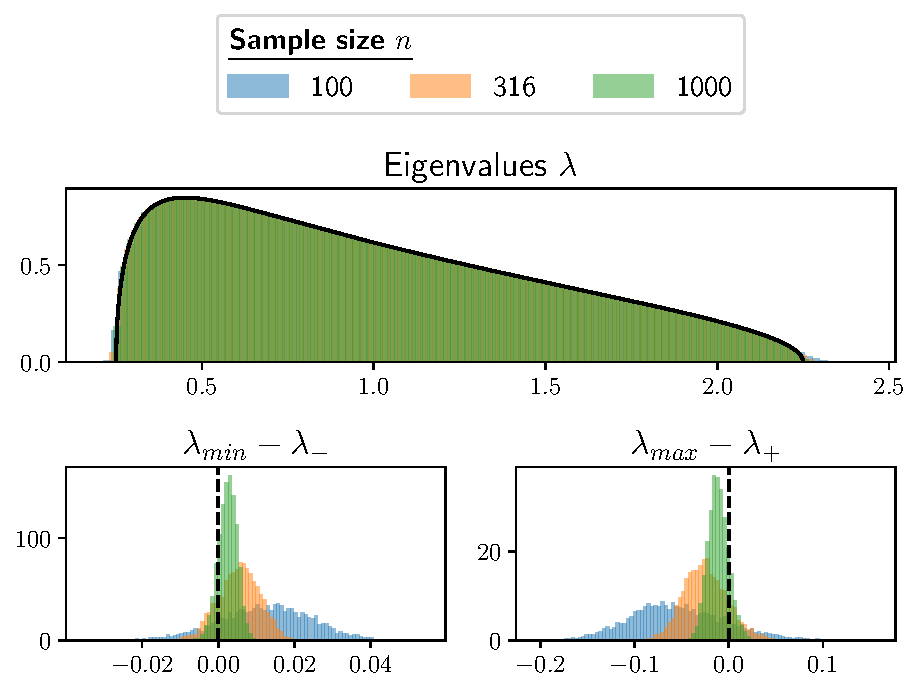
\includegraphics[width=.8\textwidth]{marchenko_pastur_alpha=0.25.pdf}\\[.5em]
        $\sigma^2=1, \quad\alpha = 0.25, \quad \lambda_{min} = \lambda_- = 0.25, \quad \lambda_{max} = \lambda_+ = 2.25$\\

    \end{frame}

    \begin{frame}{The Marchenko Pastur Law - empirically}
        \centering
        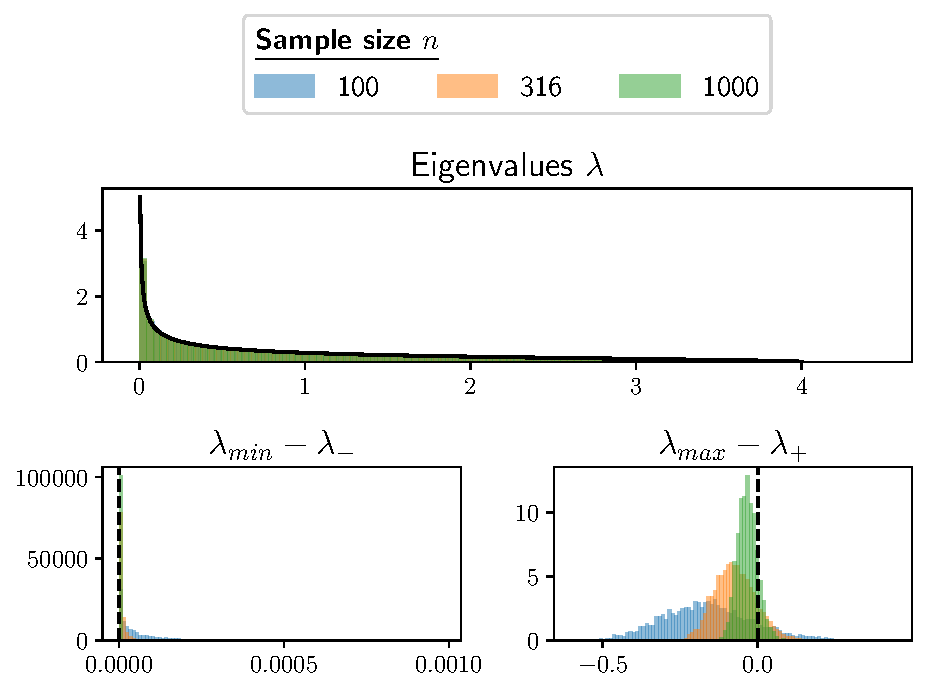
\includegraphics[width=.8\textwidth]{marchenko_pastur_alpha=1.pdf}\\[.5em]
        $\sigma^2=1, \quad\alpha = 1, \quad \lambda_{min} = \lambda_- = 0, \quad \lambda_{max} = \lambda_+ = 4$\\

    \end{frame}

    \begin{frame}{The Marchenko Pastur Law - empirically}
        \centering
        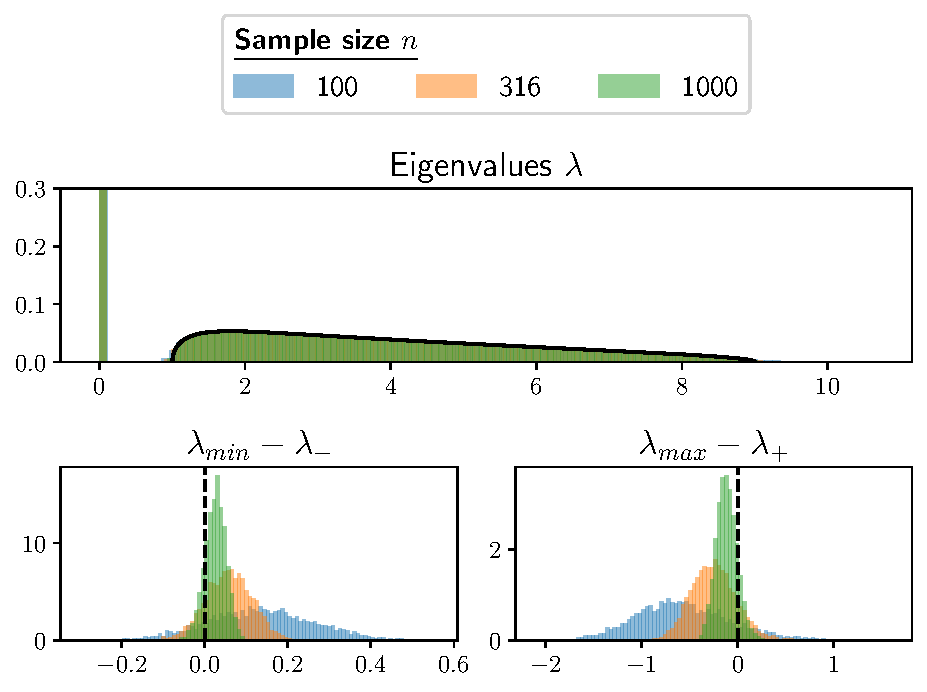
\includegraphics[width=.8\textwidth]{marchenko_pastur_alpha=4.pdf}\\[.5em]
        $\sigma^2=1, \quad\alpha = 4, \quad \lambda_{min} = \lambda_- = 1, \quad \lambda_{max} = \lambda_+ = 9$\\

    \end{frame}

\end{document}